\documentclass[conference]{IEEEtran}
% \IEEEoverridecommandlockouts
% The preceding line is only needed to identify funding in the first footnote. If that is unneeded, please comment it out.

\usepackage{cite}
\usepackage{hyperref}
\usepackage{amsmath,amssymb,amsfonts}
\usepackage{algorithmic}
\usepackage{graphicx}
\usepackage{textcomp}
\usepackage{xcolor}
\usepackage{makecell}
\usepackage{tabularx, longtable}
\usepackage{tablefootnote}

\def\BibTeX{{\rm B\kern-.05em{\sc i\kern-.025em b}\kern-.08em
    T\kern-.1667em\lower.7ex\hbox{E}\kern-.125emX}}

\begin{document}

\title{Forecasting S\&P BSE SENSEX and \\ S\&P-500 Indices Using Autoregressive Integrated Moving Average (ARIMA) Model and Prophet Library\\
	% {\footnotesize \textsuperscript{*}Note: Sub-titles are not captured in Xplore and should not be used}
	% \thanks{Identify applicable funding agency here. If none, delete this.}
}

\author{
\IEEEauthorblockN{Suraj Prakash Sharma \footnote{\textit{Amrita School of Engineering, Bengaluru}}}
	\IEEEauthorblockA{\textit{Master of Technology (M.Tech)} \\
	\IEEEauthorblockA{\textit{Data Science} \\
	\href{mailto:Sharmasurajofficial@gmail.com}{Sharmasurajofficial@gmail.com}}}
	\and
\IEEEauthorblockN{Jeyanthi R. \footnote{\textit{Amrita School of Engineering, Bengaluru}}}
	\IEEEauthorblockA{\textit{Assistant Professor (Sr. Grade)} \\
	\IEEEauthorblockA{\textit{Electronics and Communication Engineering} \\
	\href{mailto:r\_jeyanthi@blr.amrita.edu}{r\_jeyanthi@blr.amrita.edu}}}
    \and
\IEEEauthorblockN{Dr. K. Deepa \footnote{\textit{Amrita School of Engineering, Bengaluru}}}
    \IEEEauthorblockA{\textit{Assistant Professor}
	\IEEEauthorblockA{\textit{Electrical \& Electronics} \\
	\href{mailto:k\_deepa@blr.amrita.edu}{k\_deepa@blr.amrita.edu}}}
}

\maketitle

\begin{abstract}
	The study forecasts equity market benchmark indexes daily close values and capture volatility dynamics from assorted trends of S\&P SENSEX of Bombay Stock Exchange (BSE) and S\&P-500 of New York Stock Exchange (NYSE). To accomplish the objectives, use of descriptive statistics and plots related to lag, ACF, PACF were developed to understand the time-series, unit-root tests like Augmented Dickey-Fuller for stationarity, and time series models such as ARIMA and models provided by Prophet opensource library developed by Facebook were used and leveraged with hyperparameter tuning to achieve reliable performance.
	% \textbf{SARIMAX $(2, 0, 0) \times (2, 0, 0, 7)$} for S\&P BSE SENSEX and \textbf{SARIMAX $(5, 1, 1) \times (2, 0, 1, 7)$} for S\&P-500 yielded promising results with a MAPE of $4.05\%$ and $0.61\%$. 
	Prophet-based forecasting models developed for both the indices have performed better than corresponding ARIMA models when forecasting S\&P BSE SENSEX and S\&P-500, with MAPE of $1.06\%$ and $0.62\%$.
	The developed models can capture the assorted trends present in the indexes data, which can help in developing the investment strategy in short term or portfolio optimization to maximize the profits. \newline
	Although there are various studies \cite{b9} related to using ARIMA and Prophet based models for financial time series forecasting, none of them has been used to forecast the S\&P-BSE SENSEX and S\&P-500 Indexes collectively. \newline
	The results published in this study are fully reproducible and used datasets, source-codes and Google Colab \& Jupyter Notebook are available on \href{https://github.com/strikersps/Forecasting-India-and-USA-Benchmark-Indices-Using-ARIMA-and-Prophet}{GitHub} (Refer Appendix-I for GitHub Link).
\end{abstract}

\begin{IEEEkeywords}
	Efficient Market Hypothesis, Bombay Stock Exchange, New-York Stock Exchange, S\&P BSE SENSEX, S\&P-500, ADF-Test, Forecasting, ARIMA, SARIMAX, Prophet.
\end{IEEEkeywords}

\section{Introduction}

% \subsection{Description}
A lot of studies both at theoretical and empirical level have been done when it comes to figuring out what factors and variables affecting the price/value movements of securities/assets which are seen in the different segments of stock market over a given time period. Investment decisions by taking into consideration the adjusted risks play a significant role in achieving the desired returns, hence forecasting the price or the value of underlying securities/assets can help in making better investment decisions and portfolio optimization which leads to maximum returns. However, stock markets are generally known by their dynamic, complex, turbulent and volatile nature, which makes it a challenging problem to forecast the prices of securities/assets both in short and long term. Moreover, researchers and practioners have put a lot of effort on how to improve the developed models forecasting of price movements accuracy and also capture the randomness or temporal characterstics present in the financial time-series data.

According to Efficient Market Hypothesis (EMH), markets are efficient when the prices of the underlying tradeable securities completely reflect the public/private information which is directly or indirectly related to the underlying securities/assets i.e., share prices of stocks reflect all available information about companies and investors cannot beat the market indexes by stock picking \cite{b1}. Furthermore, market efficiency according to Efficient Market Hypothesis are categorized in three forms: (i) Weak, (ii) Semi-Strong, (iii) Strong.

\begin{itemize}
    \item \textbf{Weak-Form:} The price of the tradeable securities/assets will reflect the historical prices.
    \item \textbf{Semi-Strong-Form:} The price of the tradeable securities/assets will reflect the historical prices as well as the public announcements and information i.e. annual reports, share buybacks, stock splits, etc. 
    \item \textbf{Strong-Form:} The price of the tradeable securities/assets will reflect the historical prices, public announcements and private information i.e. insider trading, etc.
\end{itemize}

In this study, we have considered two benchmark indexes i.e. S\&P BSE SENSEX and S\&P 500 where S\&P BSE SENSEX is one of the flagship and benchmark indexes (other being NIFTY-50) of the Indian stock market, which is a collection of 30 publicly listed blue-chip companies and S\&P 500 is one of the flagship and benchmark indexes of the United States stock market (other being NASDAQ Composite \& Dow Jones Industrial Average (DJIA)) which is a collection of 500 largest publicly listed companies in the United States stock exchange. Moreover S\&P 500 index is one of the oldest stock market indexes in the world.

The reasons for choosing these two indexes of two different markets i.e. Indian Stock Market \& United States Stock Market for this study is because indexes of any stock market allow you to gauge the sentiment of the market, tells you about the underlying economy, and helps you to make a comparison about which market is going to do well in the future i.e. emerging market (Indian Stock Market) or developed markets (United States Stock Market) based on the trends forecasted by the respective models.

% \subsection{Problem Statement}
There are several studies in the research community which were carried out on the predictions of stock market returns using ARIMA and other powerful models especially for developed markets i.e. United States, European Markets. However, very few have focused on emerging/developing and less developed markets. This study fills the gap by forecasting S\&P BSE SENSEX (Emerging Market Index) and S\&P-500 (Developed Market Index) in order to help the investors to make a more informed decision related to their investments regarding both the markets.

% \subsection{Literature Survey}
The Efficient Markets Theory (EMT) of modern financial economics states that in an efficient market the price of tradeable security reflects all relevant information (public and private) that is available about the intrinsic value of the asset. Although the theory applies to all the different types of financial securities/assets, the discussions related to the EMT theory usually focus on one kind of security i.e. share price of a business or equity market. Financial security represents a claim on future cash flows, and thus the intrinsic value of any financial asset is the present value of the cash flows the owner of the asset expected to gain.
Theoretically, the profit opportunities represented by the existence of "undervalued” and “overvalued” securities/assets influence investor's actions in the market and their trading moves the prices of securities/assets towards the present value of future cash flows. Thus, investment analysts deploy various investment strategies but at the fundamental level, all those strategies involve a search for mispriced securities and their subsequent trading to make the market efficient and cause prices to reflect intrinsic values. Changes in the price of security in an efficient market is random because new information is either randomly favourable or unfavourable based on investors expectations hence the security prices shows a random walk behaviour. Thus in an efficient market it is impossible for an investor to realise exceptionally high risk-adjusted returns where the prices of the tradeable securities always reflect its intrinsic value \cite{b1}.

Forecasting methods for stock market returns play a pivotal role whenever an organization or an individual wants to develop/implement an investment strategy or policies or portfolio optimization algorithms to maximize profits/returns. Recent computational advancements have resulted into the development of various powerful econometric models, which have the ability to anticipate market movements/irregularities which helps in forecasting the future prices/returns of the tradeable securities \cite{b2}.

\section{Exploratory Data Analysis}
\subsection{Data \& Methodology}
The datasets collected are either by using the library or by \href{https://cutt.ly/5b6Yn9L}{Yahoo Finance website}.
% \vspace{-0.4cm}
\begin{table}[htbp]
    \renewcommand{\arraystretch}{1.5}
	\caption{Source of Datasets.}
	\begin{tabular}{| c | l | c | l |}
	\hline
		\textbf{Sr. No} & \textbf{Dataset Name} & \textbf{Time-Period} & \textbf{Source}       \\
	\hline
		1              & S\&P BSE SENSEX       & 2000-2020            & quandl library        \\
	\hline
		2              & India VIX             & 2008-2020            & investpy library      \\
	\hline
		3              & S\&P-500              & 2000-2020            & Yahoo Finance Website \\
	\hline
		4              & CBOE VIX              & 1990-2020            & investpy library \\     
	\hline
	\end{tabular}
\end{table}

India \& CBOE VIX Index datasets are used for explaining high market volatility observed during the year FY 2007-2008 \& FY 2020-2021. \newline
Jarque Bera test is one of statistcal test used to find the evidence of whether the given numerical sequence is normally distributed or not on the basis of test statistic or p-value \newline 
$H_{0}: $ The given sequence is normally distributed.\\
$H_{A}: $ The given sequence has other distribution.

Most of the financial time series data are Random Walk process and a process is said to be Random Walk if every value recorded in the during the process is a result of a random event.

Random Walk Process is governed by equations \eqref{eq:1} - \eqref{eq:3} as follows:  
\begin{align}
    P_{t} = P_{t - 1} + \epsilon_{t} \label{eq:1}\\
    P_{t} = d + P_{t - 1} + \epsilon_{t} \label{eq:2}\\
    P_{t} = P_{0} + dt + \sum_{t = 1}^{n} \epsilon_{t} \label{eq:3}
\end{align}
where   $P_{t} = $ Value of underlying series at time $t$. \\
$P_{t - 1} = $  Value of underlying series at time $t - 1$. \\
$d = $ Drift (which is just a trend like property for a random walk process, i.e.\\ $d > 0 \implies$ Upward trend and $d < 0 \implies$ downward trend).\\
$\epsilon_{t} = $ White Noise or Gaussian White Noise.

\subsection{S\&P BSE SENSEX Index EDA}
\begin{table}[htbp]
    \caption{Descriptive Statistics of S\&P BSE SENSEX Close and \%-Change Values.}
	\resizebox{\columnwidth}{!}{%
	\begin{tabular}{| c | l | p{0.2\textwidth} | p{0.2\textwidth} |}
	\hline
		\textbf{Sr.No} & \textbf{Statistics} & \textbf{Close} & \textbf{\%-Change} \\
	\hline
		1              & Mean           & $17930.2$        & $0.0525427$          \\
	\hline
		2              & Median         & $17222.6$        & $0.0952336$          \\
	\hline
		3              & Min            & $2600.12$        & $-13.1526$           \\
	\hline
		4              & Max            & $47751.3$        & $17.3393$            \\
	\hline
		5              & Std. Dev       & $11379.9$        & $1.4641$             \\
	\hline
		6              & Skewness       & $0.401981$       & $-0.13972$           \\
	\hline
		7              & Kurtosis       & $-0.875044$      & $9.65161$            \\
	\hline
		8              & Jarque Bera Test\tablefootnote{\href{https://cutt.ly/5nwffCF}{Jarque Bera Test} is used to find out whether the values are normally distributed or not.} &
		\begin{itemize}
		    \item t-statistic $= 307.514$
		    \item p-value $= 0.0$ 
		\end{itemize} &
	    \begin{itemize}
		    \item t-statistic  $ = 20257.592$
		    \item p-value  $ = 0.0$ 
		\end{itemize} \\
	\hline
	\label{tab:s_and_p_bse_sensex_decriptive_stats}
	\end{tabular}
	}
\end{table}
As p-value $< 0.05$ for Close and \%-Change values (refer Table \ref{tab:s_and_p_bse_sensex_decriptive_stats}) of S\&P-BSE SENSEX index implies that the observations recorded are not normally distributed.

\begin{figure}[htbp]
    \centering
	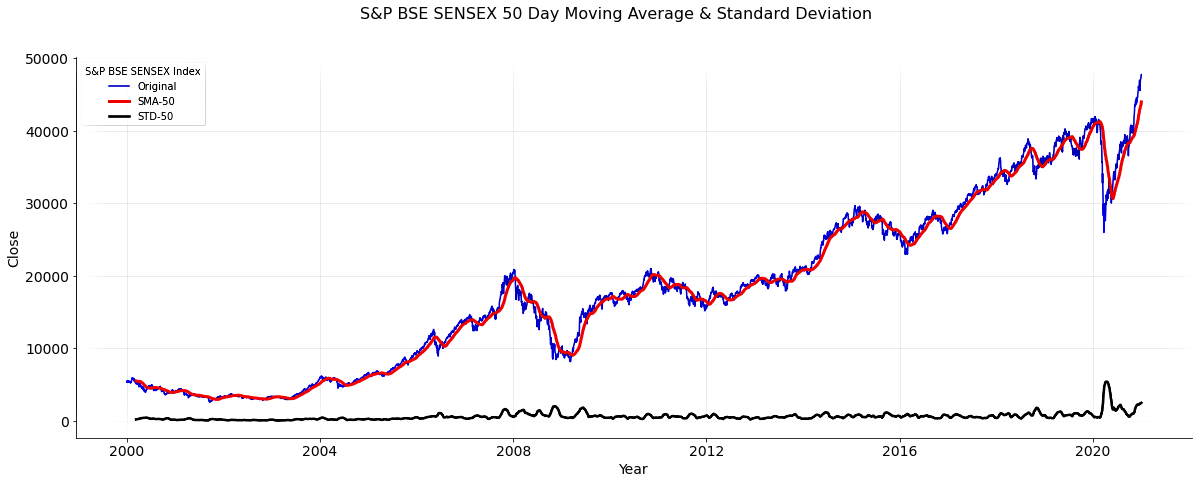
\includegraphics[width = 0.50 \textwidth]{images/SENSEX-Line-Plot.png}
	\caption{S\&P BSE SENSEX Line Plot}
	\label{fig: s_and_p_bse_sensex_line_plot}
	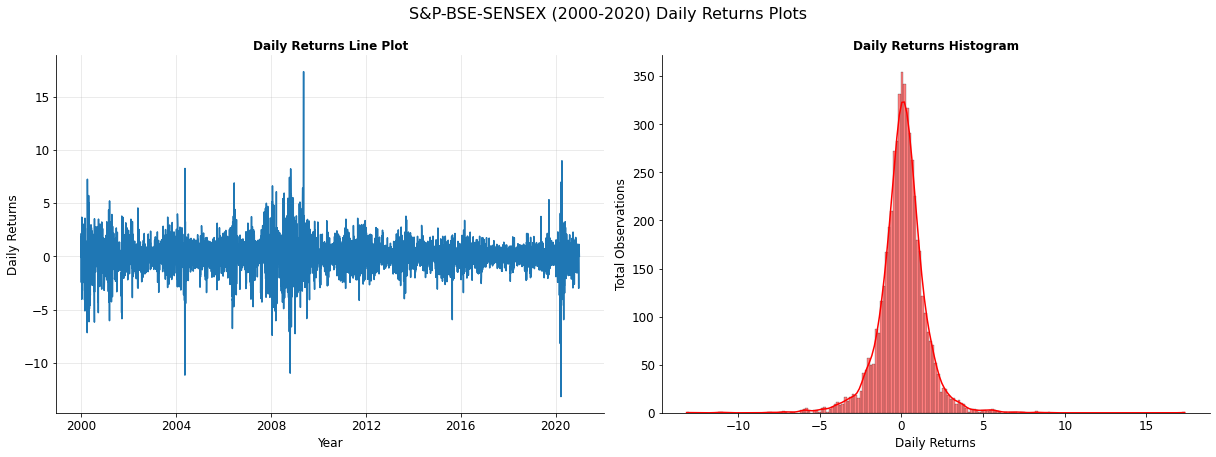
\includegraphics[width = 0.50 \textwidth]{images/SENSEX 2000-2020 Change Plot.png}
	\caption{S\&P BSE SENSEX \%-Change Plots.}
	\label{fig: s_and_p_bse_sensex_percentage_change_plot_1}
	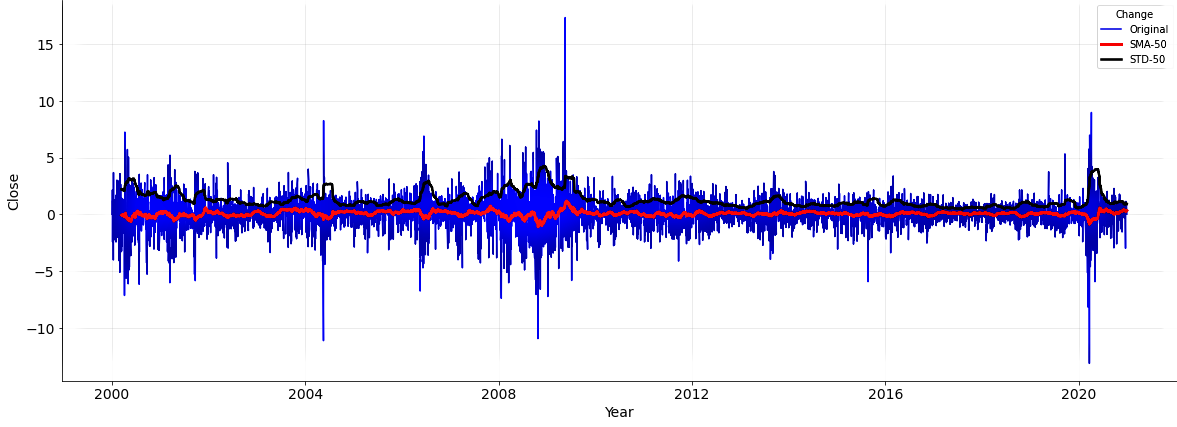
\includegraphics[width = 0.50 \textwidth]{images/BSE SENSEX White Noise Part.png}
	\caption{S\&P BSE SENSEX \%-Change (White Noise Process).}
	\label{fig: s_and_p_bse_sensex_percentage_change_plot_2}
\end{figure}
	
From Figure \ref{fig: s_and_p_bse_sensex_line_plot} it is clear that there is a trend component present and also its statistical properties like mean ($\mu$), standard deviation ($\sigma$) and variance ($s$) are dependent on time.
From Figure \ref{fig: s_and_p_bse_sensex_percentage_change_plot_1}, the \%-Change plot resembles with the white noise process and as the first difference of the given time series data (Figure \ref{fig: s_and_p_bse_sensex_percentage_change_plot_2}) is a white noise as mean ($\mu \approx 0$) and standard deviation ($\sigma$) is constant implies that the underlying time series data i.e. S\&P BSE SENSEX is a Random Walk process.

\subsection{S\&P-500 Index EDA}
Same inferences observed during the exploratory data analysis of S\&P-500 Index.
% \vspace{-0.4cm}
\begin{table}[htbp]
    \caption{Descriptive Statistics of S\&P-500 Close and \%-Change Values.}
	\resizebox{\columnwidth}{!}{%
	\begin{tabular}{| c | l | p{0.2\textwidth} | p{0.2\textwidth}|}
	\hline		
	\textbf{Sr. No} & \textbf{Statistics}   & \textbf{Close} & \textbf{\%-Change} \\
	\hline
		1              & Mean             & $1653.27$        & $0.025695$           \\
	\hline
		2              & Median           & $1386.95$        & $0.0593618$          \\
	\hline
		3              & Min              & $676.53$         & $-11.9841$           \\
	\hline
		4              & Max              & $3735.36$        & $11.58$              \\
	\hline
		5              & Std. Dev         & $673.836$        & $1.25313$            \\
	\hline
		6              & Skewness         & $1.03217$        & $-0.1538$            \\
	\hline
		7              & Kurtosis         & $0.0629593$      & $10.736$             \\
	\hline
		8              & Jarque Bera Test & 
		\begin{itemize}
		    \item t-statistic $= 938.37$
		    \item p-value $= 0.0$
		\end{itemize} & 
		\begin{itemize}
		    \item t-statistic $= 25339.39$
		    \item p-value $= 0.0$
		\end{itemize} \\
	\hline
	\label{tab: s_and_p_500_statiscal_analysis}
	\end{tabular}
	}
\end{table}
	
As p-value $< 0.05$ for Close and \%-Change values (refer Table \ref{tab: s_and_p_500_statiscal_analysis}) of S\&P-500 index implies that the observations recorded are not normally distributed.
	
\begin{figure}[htbp]
	\centering
	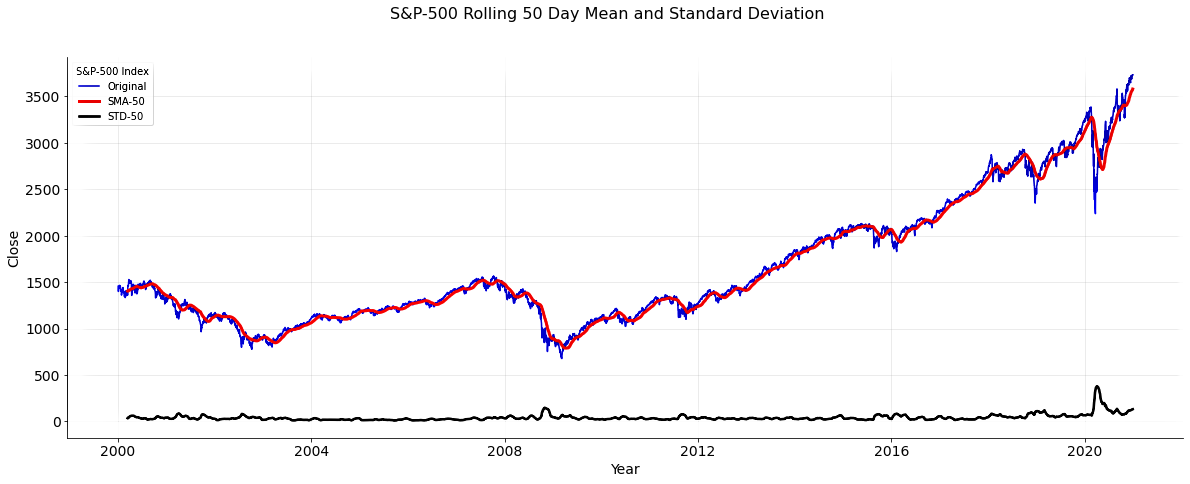
\includegraphics[width = 0.52 \textwidth]{images/S&P-500 Line Plot.png}
	\caption{S\&P-500 Index Line Plot.}
	\label{fig: s_and_p_500_index_line_plot}
	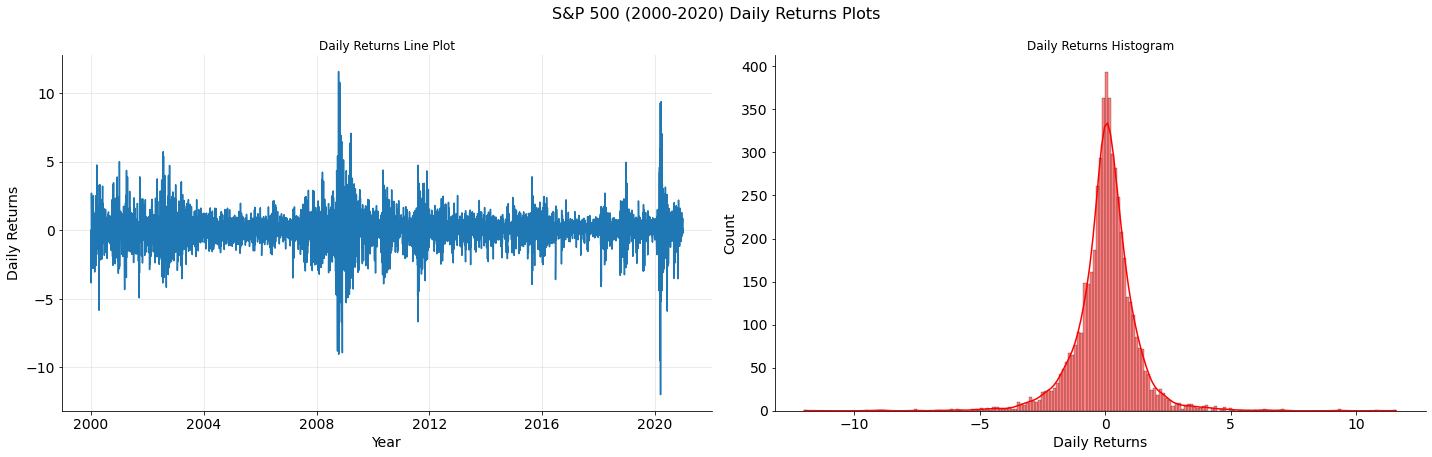
\includegraphics[width = 0.51 \textwidth]{images/S&P-500 Change Plot.png}
	\caption{S\&P-500 \%-Change Plots.}
	\label{fig: s_and_p_500_percentage_change_plot_1}
	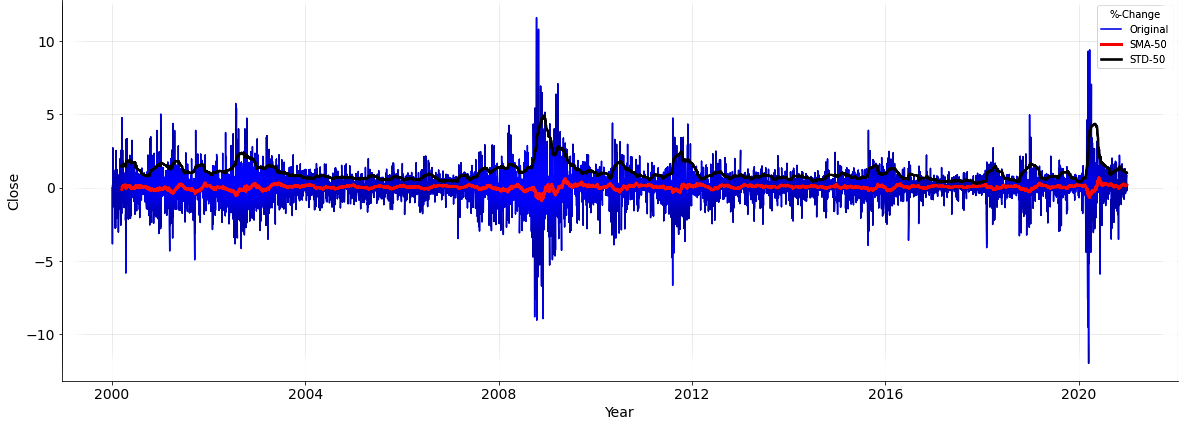
\includegraphics[width = 0.51 \textwidth]{images/S&P-500 White Noise Part.png}
	\caption{S\&P-500 \%-Change (White Noise Process).}
	\label{fig: s_and_p_500_percentage_change_plot_2}
\end{figure}
From Figure \ref{fig: s_and_p_500_index_line_plot} it is clear that there is a  trend component present in the time series data and also its statistical properties like mean ($\mu$), standard deviation ($\sigma$) and variance ($s$) are dependent on time.
From Figure \ref{fig: s_and_p_500_percentage_change_plot_1} the \%-Change plot resembles with the white noise process and as the first difference of the given time series data (Refer Figure \ref{fig: s_and_p_500_percentage_change_plot_2}) is a white noise as mean ($\mu \approx 0$) and standard deviation ($\sigma$) is constant implies that the underlying time series data i.e. S\&P-500 Index is a Random Walk process.

\subsection{VIX Indexes}
VIX Indexes allows you to measure quantitatively in real-time, near-term volatility expectations of the market from the perspective of the future and options market. Fig. \ref{fig:india_vix_index} shows the India VIX Index and Fig. \ref{fig:cboe_vix_index} shows the CBOE VIX Index.

The CBOE Volatility Index also known as the stock market’s “fear gauge” and reflects the expectations of investors on the presence of volatility in the S\&P-500 index (SPX) over the next 30 days and computed based on prices of put and call options on the S\&P 500 index (SPX).
India VIX for measuring the volatility in Indian Equity Market was launched in 2007 and computed by NSE where the computation of the India VIX values is based completely on the order book of NIFTY Futures and Options (F\&O). For the computation of India VIX values, the best bid-ask excerpt of near ($\sigma_{1}$) and next-month ($\sigma_{2}$) NIFTY options contracts traded on the F\&O segment of NSE are considered \cite{b4}. \newline
The equations used for the computation of India VIX is:
\begin{align}
    \sigma^{2} = \frac{2}{T} \sum_{i}\frac{\Delta K_{i}}{K_{i^{2}}}e^{{RT}}Q(K_{i}) - \frac{1}{T}\Big[\frac{F}{k_{0}} - 1\Big]^2 \label{eq: 4}
\end{align}
where: \newline
    $\sigma = $ India VIX $/100 \implies$ India VIX $ = \sigma \times 100$. \newline
    $T =$ Time to expiration. \newline
    $K_{i} = $ Strike price of $i^{th}$ out of money option; a call if $K_{i} > F$ and a put if $K_{i} < F$. \newline
    $\Delta K_{i} =$ Interval between strike prices- half the distance between the strike on either side of $K_{i}$. 
    \begin{align}
        \Delta K{i} = \frac{K_{i + 1} - K_{i - 1}}{2} \label{eq: 5}
    \end{align}
    (NOTE: $\Delta K$ for the lowest strike is simply the difference between the lowest strike and the next higher strike. Likewise, $\Delta K$ for the highest strike is the difference between the highest strike and the next lower strike).\newline
    $R =$ Risk-free interest rate of expiration.
    $Q(K_{i}) =$ Midpoint of bid-ask quote for each option contract with strike $K_{i}$. \newline
    $F =$ Forward index taken as the latest price of NIFTY future contract of corresponding expiry. \newline
    $K_{0} =$ First strike below the forward index level $F$. \newline
    
    India VIX values are evaluated by individually computing the near month ($\sigma_{1}$) and next month ($\sigma_{2}$) VIX values with time to expiration of $T_{1}$ and $T_{2}$ respectively and then ${\sigma}^{2}$ value is arrived at by interpolating $\sigma_{1}$ and $\sigma_{2}$ according to \ref{eq:6}:
    \begin{align}
        {\sigma}^{2} = \Big\{T_{1}{\sigma_{1}}^{2}\Big[\frac{N_{T_{2}} - N_{30}}{N_{T_{2}} - N_{T_{1}}}\Big] + T_{2}{\sigma_{2}}^{2}\Big[\frac{N_{30} - N_{T_{1}}}{N_{T_{2}} - N_{T_{1}}}\Big]\Big\} \times \frac{N_{365}}{N_{30}} \label{eq:6}
    \end{align}
where: \newline
    $N_{T_{1}} =$ Total minutes to expiration of near month options $= 12960$. \newline
    $N_{T_{2}} =$ Total minutes to expiration of next month options $= 53280$. \newline
    $N_{30} =$ Total minutes in $30$ days $= 43200$. \newline
    $N_{365} =$ Total minutes in $365$ days $= 525600$. \newline
    
India VIX ($\sigma^{2}$) measures the expected market volatility over the next $30$ calendar days. Higher the India VIX values, higher the expected volatility, and vice-versa.
% For more detailed information on how the values of India VIX are computed, please refer the white paper published by National Stock Exchange (NSE) \cite{b4} on how the computation is done with examples.

% The index is also refered as "investor fear index", the CBOE VIX is a measure of the implied volatility of the SPX, and is observed to be correlated with the 30-day realized volatility of the SPX. Changes in the CBOE VIX are observed to be negatively correlated with changes in the SPX.

% The CBOE Volatility Index (VIX) quantitatively measures the market's expectations for the relative strength of near-term price changes of the S\&P 500 index (SPX) because it's derived from the prices of SPX index options with near-term expiration dates, it generates a $30$-day forward projection of volatility.

The interesting insights from Fig. \ref{fig:india_vix_index} and Fig. \ref{fig:cboe_vix_index} are in the FY-2009 and FY-2021, the volatility observed in the both India \& USA equity markets are very high because of Global Financial Crisis in FY-2009 due to crash of Mortgage market in the USA and in FY-2021 due to COVID-19 great lockdown and the panic caused by the fear of recession in investors.

\begin{figure}[htbp]
	\centering
	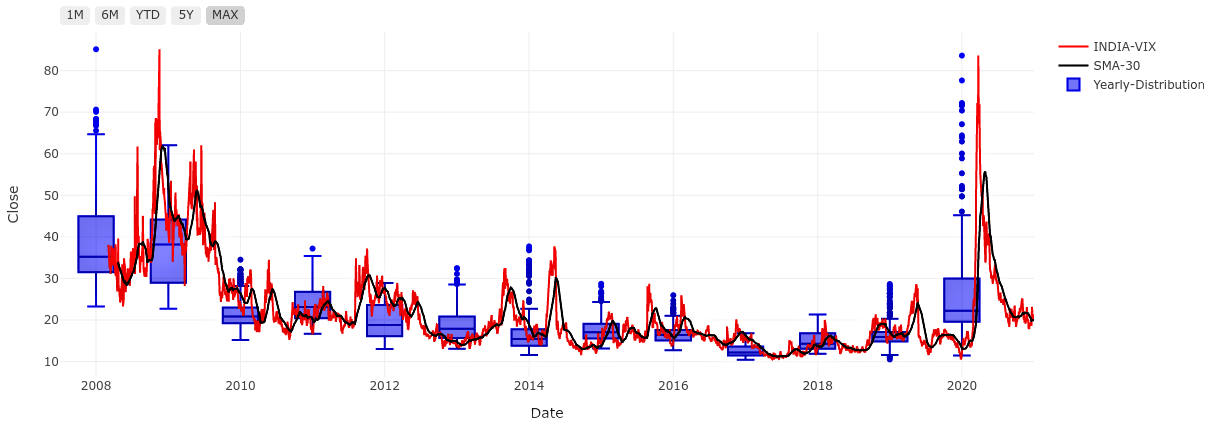
\includegraphics[width = 0.52 \textwidth]{images/INDIA-VIX (2008-2020).png}
	\caption{India VIX Index (2008-2020) Plot.}
	\label{fig:india_vix_index}
	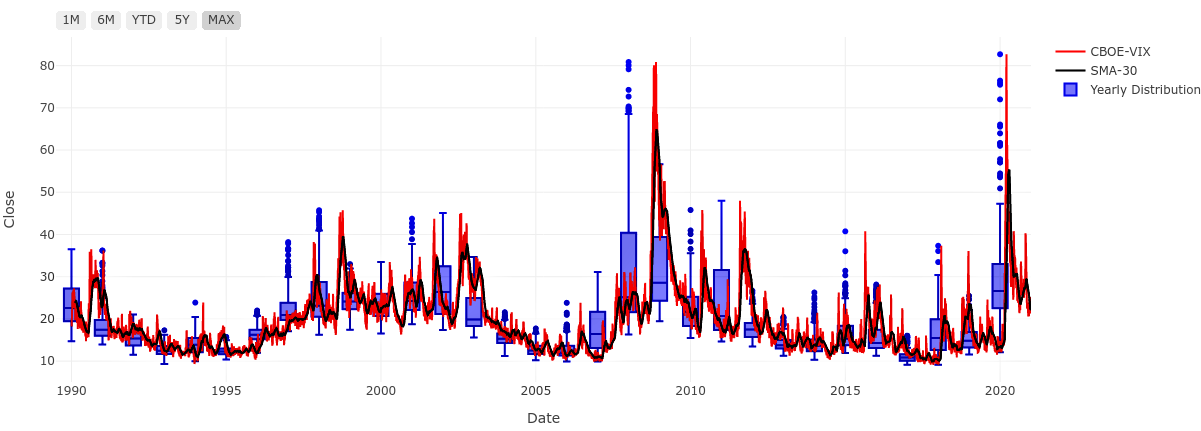
\includegraphics[width = 0.52 \textwidth]{images/CBOE-VIX.png}
	\caption{CBOE VIX Index (1990-2020) Plot.}
	\label{fig:cboe_vix_index}
\end{figure}

For both the indexes i.e. S\&P BSE SENSEX and S\&P-500 the Close value ACF plots (Fig. 9 and Fig. 11) is unity ($\approx 1$) for short-term lags and decays down to $0$ at $\approx 1900^{th}$ lag. This is one of the property of the Random Walk Process in which if the number of observations are high then autocorrelation coefficient ($\rho_{k}$) is almost unity i.e. extremely high auto-correlations that does not decreases exponentially as lag increases ($k$) beacause the autocorrelation coefficient ($\rho_{k}$) of random walk process is dependent on time ($t$) derived as follows:

\begin{align}
\rho_{k}(t) = \frac{Cov(x_{t}, x_{t+k})}{\sqrt{Var(x_{t}) \times Var(x_{t + k})}} \label{eq: 4}& \\ = \frac{t\;\sigma^{2}}{\sqrt{t\;\sigma^{2}\times(t + k)\times \sigma^{2}}} \label{eq: 5}
\end{align}
Rearranging the terms will give the following equation for autocorrelation coefficient ($\rho_{k}$) for a random walk process:
\begin{align}
\rho_{k} = \frac{1}{\sqrt{1 + (k / t)}} \label{eq: 6}
\end{align}
From equation \eqref{eq: 6}, autocorrelation coefficient ($\rho_{k}$) is inversely related to time ($t$) which is why autocorrelation coefficient ($\rho_{k}$) value was unity $\approx 1$ for shorter time lags in figure \ref{fig: s_and_p_bse_sensex_acf_and_pcf_plots} and \ref{fig: s_and_p_500_acf_and_pacf_plots}.

\onecolumn
\subsection{ACF and PACF Plots}
\begin{figure}[htbp]
	\centering
	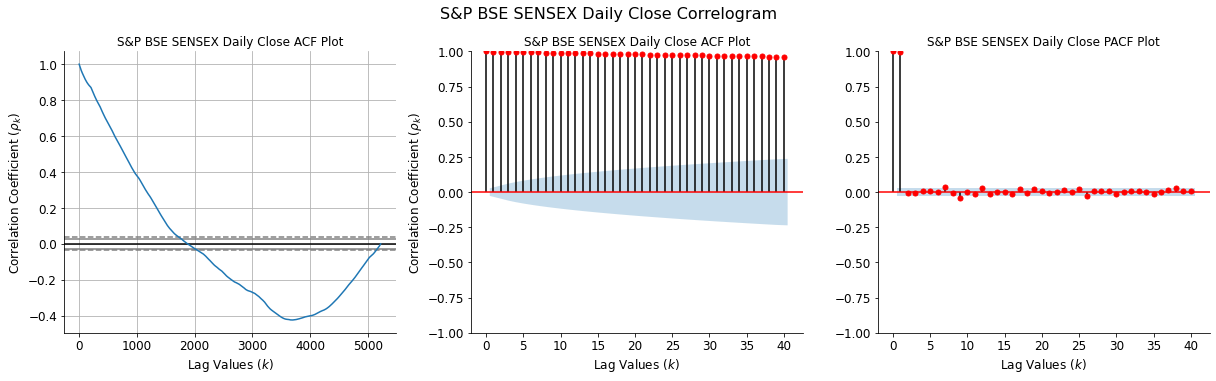
\includegraphics[width = 0.78 \textwidth]{images/SENSEX ACF and PACF Plot.png}
	\caption{S\&P BSE SENSEX ACF and PACF Plots.}
	\label{fig: s_and_p_bse_sensex_acf_and_pcf_plots}
	
	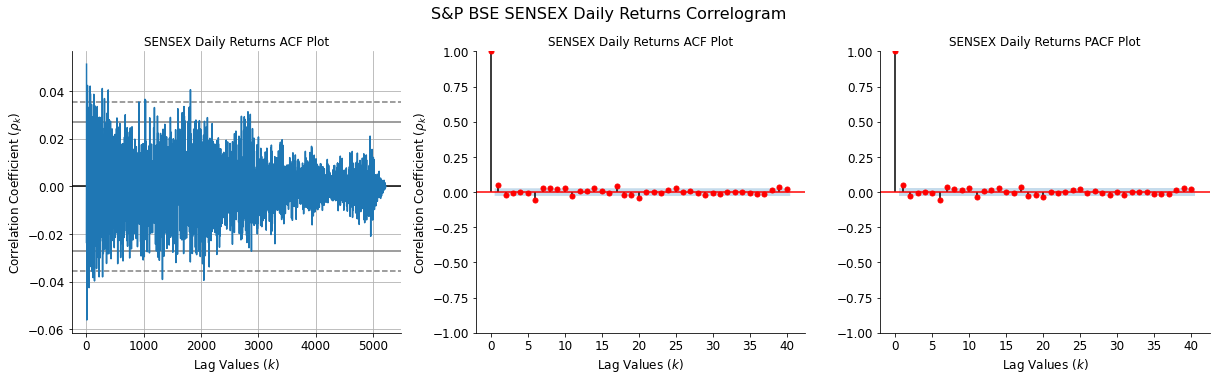
\includegraphics[width = 0.78 \textwidth]{images/SENSEX Change ACF, PACF Plots.png}
	\caption{S\&P BSE SENSEX \%-Change ACF and PACF Plots.}
	\label{fig: s_and_p_bse_sensex_percentage_change_acf_and_pacf_plots}
	
	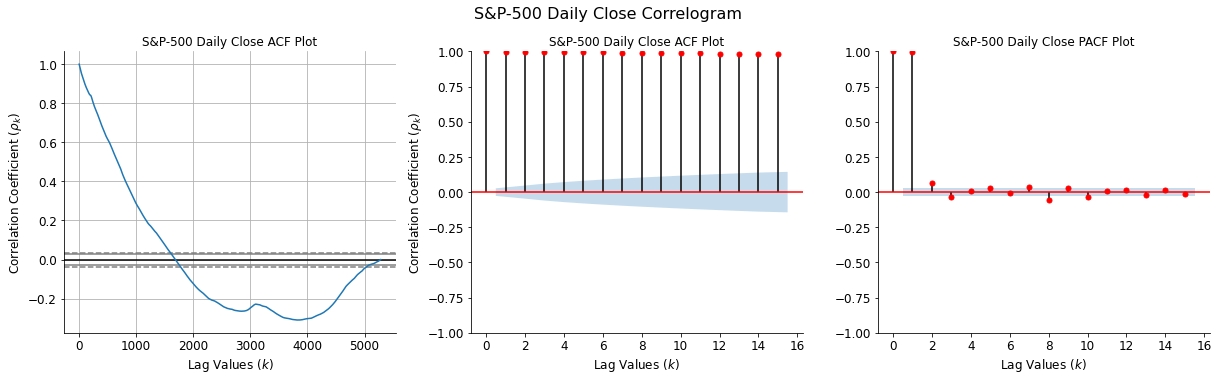
\includegraphics[width = 0.78 \textwidth]{images/S&P-500 ACF, PACF Plots.png}
	\caption{S\&P-500 ACF and PACF Plots.}
	\label{fig: s_and_p_500_acf_and_pacf_plots}
	
	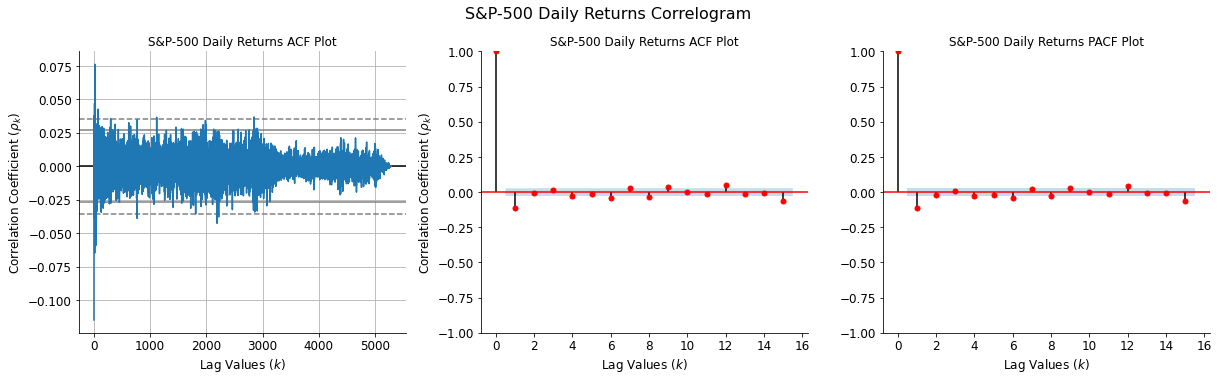
\includegraphics[width = 0.78 \textwidth]{images/S&P-500 Change ACF PACF Plot.png}
	\caption{S\&P-500 \%-Change ACF and PACF Plots.}
	\label{fig: s_and_p_500_percentage_change_acf_and_pacf_plots}
\end{figure}

For both the indexes i.e. S\&P BSE SENSEX and S\&P-500 the \%-Change ACF plot in figure \ref{fig: s_and_p_bse_sensex_percentage_change_acf_and_pacf_plots} and \ref{fig: s_and_p_500_percentage_change_acf_and_pacf_plots} doesn't show any statistically significant correlation at lags $k$ and $95\%$ of the spikes in both the ACF plots are in the range of $\pm 2/\sqrt{T}$ where $T$ represents the number of observations which implies the underlying \%-Change sequence is a white noise process.

\twocolumn
\section{Statistical Tests for Stationarity}
\subsection{Augmented Dickey Fuller Statistical Test}
Augmented Dickey Fuller (ADF) test is one of the unit root tests to check the stationarity of the timeseries data through hypothesis testing.

$H_{0}$: Given time series data is non-stationarity $\implies$ Time series data has time dependent statistical properties i.e. mean, variance, auto-correlation etc present in it.

$H_{A}:$ Given time series data is stationary $\implies$ Time series data doesn't have any time dependent statisitcal properties present in it. \newline
If the p-value obtained is $\le 0.05 \implies$ Reject the $H_{0}$ otherwise $\implies$ Failed to Reject $H_{0}.$ \newline

Tables \ref{tab: s_and_p_bse_sensex_close_value_adf_test_results}, \ref{tab: s_and_p_500_percentage_close_value_adf_test}, \ref{tab: s_and_p_500_close_value_adf_test}, and \ref{tab: s_and_p_500_percentage_close_value_adf_test} shows the results of Augmented Dickey Fuller Statistical Test performed on both the indexes.

\begin{table}[htbp]
	\caption{S\&P BSE SENSEX Close Value ADF Test Results.}
	\begin{tabular}{|c|c|c|c|c|}
		\hline
		\textbf{Sr.No} & \textbf{Data} & \textbf{t-statistic} & \textbf{p-value} & \textbf{Verdict}        \\
		\hline
		1              & Close Values  & $0.688133$           & $0.688133$       & Failed to Reject $H_{0}$. \\
		\hline
	\end{tabular}
	\label{tab: s_and_p_bse_sensex_close_value_adf_test_results}
\end{table}

As p-value obtained i.e. $0.998199 > 0.05 (\alpha) \implies$ Failed to Reject $H_{0} \implies$ S\&P BSE SENSEX Close values is \textbf{non-stationary} (Refer: Table \ref{tab: s_and_p_bse_sensex_close_value_adf_test_results}).

\begin{table}[htbp]
	\caption{S\&P BSE SENSEX \%-Change Values ADF Test Results.}
	\centering
	\begin{tabular}{|c|c|c|c|c|}
		\hline
		\textbf{Sr.No} & \textbf{Data}    & \textbf{t-statistic} & \textbf{p-value}        & \textbf{Verdict} \\
		\hline
		1              & \%-Change Values & $-16.081$            & $5.390 \times 10^{-29}$ & Reject $H_{0}$.    \\
		\hline
	\end{tabular}
	\label{tab: s_and_p_bse_sensex_percentage_change_value_adf_test}
\end{table}
As p-value obtained i.e. $5.389647 \times 10^{-27} << 0.05 (\alpha) \implies$ Reject the $H_{0} \implies$ S\&P BSE SENSEX \%-Change values is \textbf{stationary} Refer (Table \ref{tab: s_and_p_bse_sensex_percentage_change_value_adf_test}).

\begin{table}[htbp]
	\caption{S\&P-500 Close Value ADF Test Results.}
	\begin{tabular}{|c|c|c|c|c|}
		\hline
		\textbf{Sr.No} & \textbf{Data} & \textbf{t-statistic} & \textbf{p-value} & \textbf{Verdict}        \\
		\hline
		1              & Close Values  & $1.631761$           & $0.99795$        & Failed to Reject $H_{0}$. \\
		\hline
	\end{tabular}
	\label{tab: s_and_p_500_close_value_adf_test}
\end{table}
As p-value obtained i.e. $0.99795 > 0.05 (\alpha) \implies$ Failed to Reject $H_{0} \implies$ S\&P-500 Close values is \textbf{non-stationary} (Refer Table \ref{tab: s_and_p_500_close_value_adf_test}).
	
\begin{table}[htbp]
	\centering
	\caption{S\&P-500 \%-Change Values ADF Test Results.}
	\begin{tabular}{|c|c|c|c|c|}
		\hline
		\textbf{Sr.No} & \textbf{Data}    & \textbf{t-statistic} & \textbf{p-value}        & \textbf{Verdict} \\
		\hline
		1              & \%-Change Values & $-13.742$            & $1.095 \times 10^{-25}$ & Reject $H_{0}$.    \\
		\hline
	\end{tabular}
	\label{tab: s_and_p_500_percentage_close_value_adf_test}
\end{table}
As p-value obtained i.e. $1.094051 \times 10^{-25} << 0.05 (\alpha) \implies$ Reject the $H_{0} \implies$ S\&P-500 \%-Change values is \textbf{stationary} (Refer Table \ref{tab: s_and_p_500_percentage_close_value_adf_test}).

\section{Estimating Parameters of Models}
Various time-series models have a regressive structure inbuilt, so it becomes important to establish a general class of time-series models called Autoregressive Integrated Moving Average (ARIMA), also known as Box-Jenkins models due to systematic approach of identifying, fitting, checking and leveraging ARIMA models which was popularized by George Box and Gwilym Jenkins in 1976.
ARIMA models are an extension of ARMA models when dealing with non-stationary time-series data i.e. when the statistical attributes (mean, variance, standard deviation) of time-series data change with time. \newline
Mathematically ARIMA models are represented as $ARIMA(p, d, q)$ where $p = $ order of AR process, $q = $ order of MA process and $d = $ order of differencing.
The model used in this study is Seasonal ARIMA (SARIMA) but as there is requirement for exposing the SARIMA model to exogenous features i.e. those features which are not used to fit the model but have an influence on the model forecast. Hence, the model used is SARIMAX where X represents the set of exogenous features.

The exogenous variables (X) used for the SARIMAX model are all extracted from the dataset itself i.e. standard deviation and moving averages for 3, 7, 30, 50, 100 days of the index high and close values for each trading day and no external variables such as VIX, GDP, CPI, WPI and other sets of financial or economic data are used as exogenous variables for forecasting.

For Prophet\cite{b6} library based predictions, there is no need to estimate parameters because the library has abstracted that process and same set of exogenous features are used as in the SARIMAX during the training and forecasting of Prophet models.

\subsection{S\&P BSE SENSEX Index}
Estimated hyperparameters of SARIMAX $(p, d, q) \times (P, D, Q, M)$ are: SARIMAX $(2, 0, 1) \times (2, 0, 0, 7)$ with an AIC $\approx 64126.053$ (Refer Table \ref{tab:sensex_hyperparameters_tunning_result_table} and Figure \ref{fig:sensex_sarimax_parameter_estimation_report} in Appendix-II for more details related to coefficients of SARIMAX equations determined through step wise search method).

\subsection{S\&P-500 Index}
Estimated hyperparameters of SARIMAX $(p, d, q) \times (P, D, Q, M)$ are: SARIMAX $(5, 1, 1) \times (2, 0, 1, 7)$ with an AIC $\approx 35713.686$ (Refer Table \ref{tab:s_and_p_500_hyperparameters_tunning_results_table} and Figure \ref{fig:s_and_p_500_parameter_estimation_report} in Appendix-II for more details related to coefficients of SARIMAX equations determined through step wise search method).

\onecolumn
\section{Validation For Actual and Forecasted Values}
\subsection{S\&P BSE SENSEX Index}
The following graphs shows the performance of the models (SARIMAX and Prophet) on validation data of S\&P BSE SENSEX.
\begin{figure}[htbp]
	\centering
	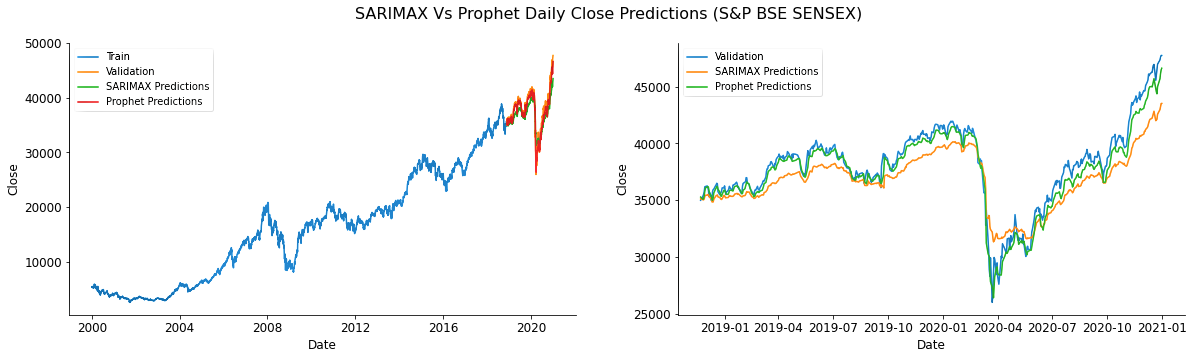
\includegraphics[width = \textwidth]{images/SARIMAX-Prophet-SENSEX-Predictions.png}
	\caption{SARIMAX and Prophet Model Predictions on Validation Data for S\&P BSE SENSEX.}
	\label{fig:sarimax_prophet_results_sensex_index}
\end{figure}

\begin{table}[htbp]
	\setlength{\tabcolsep}{20pt}
	\renewcommand{\arraystretch}{1.2}
	\centering
	\caption{SARIMAX and Prophet Error Metric Values.}
	\begin{tabular}{| c | c | c | c | c | c |}
		\hline
		\textbf{Model} & \textbf{MAE} & \textbf{MSE} & \textbf{RMSE} & \textbf{R2-Score} & \textbf{MAPE} \\
		\hline
		SARIMAX        & 1553.14     & $3.39 \times 10^{6}$ & 1839.91      & 0.7314          & $4.05 \%$     \\
		\hline
		Prophet        & 611.33      & $5.998 \times 10^{5}$ & 774.44       & 0.95             & $1.60\%$      \\
		\hline
	\end{tabular}
	\label{tab:s_and_p_sensex_model_evaluation_metric_table}
\end{table}

\subsection{S\&P-500 Index}
The following graphs shows the performance of the models (SARIMAX and Prophet) on validation data of S\&P-500 Index.

\begin{figure}[htbp]
	\centering
	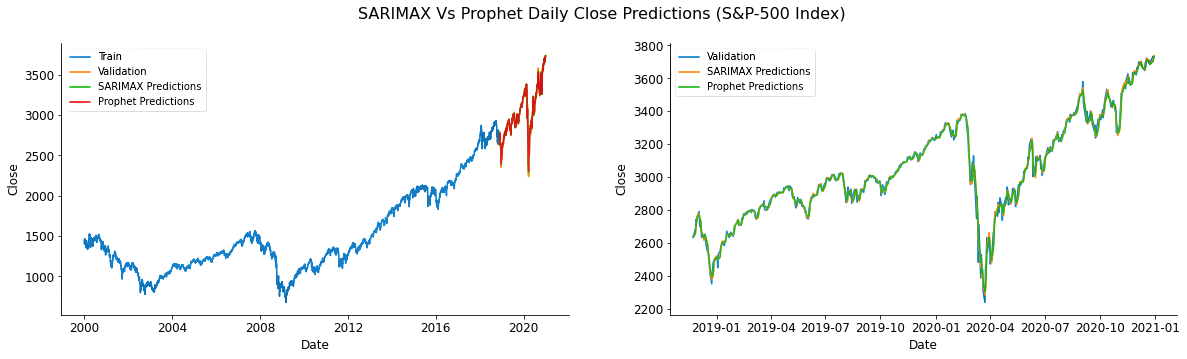
\includegraphics[width = \textwidth]{images/SARIMAX-Prophet-S&P-500-Predictions.png}
	\caption{SARIMAX and Prophet Model Predictions on Validation Data for S\&P-500.}
	\label{fig: sarimax_prophet_results_for_s_and_p_500_index}
\end{figure}

\begin{table}[htbp]
	\setlength{\tabcolsep}{20pt}
	\renewcommand{\arraystretch}{1.5}
	\centering
	\caption{SARIMAX and Prophet Error Metric Values.}
	\begin{tabular}{|c | c | c | c | c | c |}
	\hline
	\textbf{Model} & \textbf{MAE} & \textbf{MSE} & \textbf{RMSE} & \textbf{R2-Score} & \textbf{MAPE} \\
	\hline
	SARIMAX        & 18.189       & 755.416      & 27.484822     & 0.991685          & $0.62 \%$     \\
	\hline
	Prophet        & 18.452       & 770.787      & 27.764        & 0.991516          & $0.63\%$      \\
	\hline
	\end{tabular}
	\label{tab: s_and_p_500_model_evaluation_metric_table}
\end{table}

\twocolumn
\section{Findings from the Study}

From Table \ref{tab:s_and_p_sensex_model_evaluation_metric_table} and \ref{tab: s_and_p_500_model_evaluation_metric_table}, we concluded that SARIMAX $(2, 0, 0) \times (2, 0, 0, 7)$ for S\&P BSE SENSEX and SARIMAX $(5, 1, 1) \times (2, 0, 1, 7)$ for S\&P-500 yielded reliable results with a Mean Average Precision Error (MAPE) of $4.05\%$ and $0.61\%$. Prophet has performed better than both the SARIMAX models when forecasting S\&P BSE SENSEX and S\&P-500 with Mean Average Precision Error (MAPE) of $1.06\%$ and $0.62\%$. \newline
However, from Figure \ref{fig:sarimax_prophet_results_sensex_index} and Figure \ref{fig: sarimax_prophet_results_for_s_and_p_500_index} there is a significant difference in actual and predicted values on a daily basis, but the models (SARIMAX and Prophet) are able to capture the assorted trends present in the indexes data. \newline

From the application perspective, these models can be used as an approximate technical indicator of what values the indexes would take or can be used to determine the approximate trends of market indexes in short term in order to manage/optimize the portfolios to maximize the profits.

\section{Conclusions}
The volatility which was observed during the Global Financial Crisis of 2008, the same nature/level of volatility was observed in the Crash of 2020 because of COVID-19 in both the equity markets i.e. United States of America and India. \newline

The markets not only tells us the sentiment of the investor in the short-term as a reflection of the information available but also gives us an idea about what are the variables which plays a major role like Budget Announcements, Stimulus Plans, Government Policies, Foreign Direct Investments (FDIs), Foreign Institutional Investors (FIIs), Mergers and Acquisitions (M\&A) etc to move the market in either direction, but in long term, only those stocks/equities/securities are wealth creators which represents a high-quality business which is managed or run by high-quality and experienced management.

Both the markets i.e. Developed \& Emerging markets have rebounded/recovered quickly i.e. in approximately 6-7 months after the COVID-19 led market crash which is the fastest recovery historically as it takes at least 2 years for the markets normally to recover to their early highs.

\section{Future Work}
In addition to forecasting the closing values of indexes, it will also be more strategic to also forecast the $\beta$ values i.e. measure of risk with respect to benchmark indices or broader market indices \cite{b3}.

Adding more exogenous variables like P/E ratio, P/B ratio, Shared Traded, CPI, WPI, GDP, etc as external features in the dataset can help in building a more robust and reliable forecasting model.

\begin{thebibliography}{00}
	\bibitem{b1} Fama, Eugene F. “Efficient Capital Markets: A Review of Empirical Work.” Journal of Finance 25, no. 2 (1970): 383–417.
	
	\bibitem{b2} Madhavi Latha Challa \& Venkataramanaiah Malepati \& Siva Nageswara Rao Kolusu, 2020. S\&P BSE Sensex and S\&P BSE IT return forecasting using ARIMA, Financial Innovation, Springer, Southwestern University of Finance and Economics, vol. 6(1), pages 1-19, December.
	
	\bibitem{b3} Challa, M.L., Malepati, V. \& Kolusu , S.N.R. Forecasting risk using autoregressive integrated moving average approach: an evidence from S\&P BSE Sensex. Financ Innov 4, 24 (2018).
	
	\bibitem{b4} National Stock Exchange (NSE): The India VIX White paper. Available: \href{https://www1.nseindia.com/content/indices/white\_paper\_IndiaVIX.pdf}{https://www1.nseindia.com/content/indices/white\_paper\_IndiaVIX.pdf}
	
	\bibitem{b5} Manimaran, P. \& Panigrahi, Prasanta K. \& Parikh, Jitendra C., 2008. "Difference in nature of correlation between NASDAQ and BSE indices," Physica A: Statistical Mechanics and its Applications, Elsevier, vol. 387(23), pages 5810-5817.
	
	\bibitem{b6} Taylor SJ, Letham B. 2017. Forecasting At Scale. PeerJ Preprints.
	
	\bibitem{b7} Emir Zunic \& Kemal Korjenic \& Kerim Hodzic \& Dzenana Donko, 2020. "Application of Facebook's Prophet Algorithm for Successful Sales Forecasting Based on Real-world Data," Papers 2005.07575, arXiv.org.
	
	\bibitem{b8} L. Menculini, A. Marini, M. Proietti, A. Garinei, A. Bozza, C. Moretti, and M. Marconi, “Comparing Prophet and Deep Learning to ARIMA in Forecasting Wholesale Food Prices,” Forecasting, vol. 3, no. 3, pp. 644–662, Sep. 2021 [Online].
	
	\bibitem{b9} A. Garlapati, D. R. Krishna, K. Garlapati, N. m. Srikara Yaswanth, U. Rahul and G. Narayanan, Stock Price Prediction Using Facebook Prophet and Arima Models, 2021 6th International Conference for Convergence in Technology (I2CT), 2021, pp. 1-7.
	
\end{thebibliography}

\onecolumn
\appendix
\subsection{Appendix-I}
\begin{itemize}
    \item Interactive plots, source codes, Google Colab \& Jupyter Notebook are available and accessible on GitHub.
    \item \textbf{GitHub Link:} \href{https://github.com/strikersps/Forecasting-BSE-SENSEX-and-S-and-P-500-Using-ARIMA-and-Prophet}{https://github.com/strikersps/Forecasting-BSE-SENSEX-and-S-and-P-500-Using-ARIMA-and-Prophet}
\end{itemize}

\subsection{Appendix-II}
Results of stepwise search method for choosing the best $SARIMAX(p, d, q) \times (P, D, Q)$ model with the minimum AIC value after exploring various permutations of $p, d, q$ and $P, D, Q$ hyper-parameter values with $m = 7$ for S\&P BSE SENSEX and S\&P-500 benchmark indexes are tabulated in \ref{tab:sensex_hyperparameters_tunning_result_table} and \ref{tab:s_and_p_500_hyperparameters_tunning_results_table}. The value of $m$ i.e. frequency represents how many observations/cycle which normally a year but sometimes it cab be an hour, a day, a week, a month etc depending upon how you want to capture the seasonality in the given timeseries data. $\infty$ value for AIC in the Table \ref{tab:sensex_hyperparameters_tunning_result_table} represents that the AIC values were not converging for the choosen set of model hyperparameters.

\begin{table}[htbp]
    \setlength{\tabcolsep}{20pt}
    \renewcommand{\arraystretch}{1.2}
    \centering
    \caption{Hyperparameter Optimization Results For S\&P BSE SENSEX $SARIMAX(p, d, q) \times (P, D, Q)[m]$}
    \begin{tabular}{|c|c|c|c|}
        \hline
        Sr. No & Model Parameters & AIC & Time-Taken (In Seconds) \\
        \hline
        1 & $SARIMAX(2, 0, 2) \times (1, 0, 1)[7]$ & $66300.235$ & $83.78\;sec$ \\
        \hline
        2 & $SARIMAX(0, 0, 0) \times (0, 0, 0)[7]$ & $67521.064$ & $5.64\;sec$ \\
        \hline
        3 & $SARIMAX(1, 0, 0) \times (1, 0, 0)[7]$ & $\infty$ &
        $58.97\;sec$ \\
        \hline
        4 & $SARIMAX(0, 0, 1) \times (0, 0, 1)[7]$ & $68100.858$ & $65.65\;sec$ \\
        \hline
        5 & $SARIMAX(2, 0, 2) \times (0, 0, 1)[7]$ & $66595.465$ & $74.65\;sec$ \\
        \hline
        6 & $SARIMAX(2, 0, 2) \times (1, 0, 0)[7]$ & $66201.139$ & $70.81\;sec$ \\
        \hline
        7 & $SARIMAX(2, 0, 2) \times (0, 0, 0)[7]$ & $66324.432$ & $45.04\;sec$ \\
        \hline
        8 & $SARIMAX(2, 0, 2) \times (2, 0, 0)[7]$ & $65079.644$ & $118.87\;sec$ \\
        \hline
        9 & $SARIMAX(2, 0, 2) \times (2, 0, 1)[7]$ & $66059.787$ & $127.97\;sec$ \\
        \hline
        10 & $SARIMAX(1, 0, 2) \times (2, 0, 0)[7]$ & $66159.509$ & $118.06\;sec$ \\
        \hline
        11 & $SARIMAX(2, 0, 1) \times (2, 0, 0)[7]$ & $63798.806$ & $121.01\;sec$ \\
        \hline
        12 & $SARIMAX(2, 0, 1) \times (1, 0, 0)[7]$ & $65989.971$ & $67.07\;sec$ \\
        \hline
        13 & $SARIMAX(2, 0, 1) \times (2, 0, 1)[7]$ & $64092.022$ & $120.76\;sec$ \\
        \hline
        14 & $SARIMAX(2, 0, 1) \times (1, 0, 1)[7]$ & $65550.925$ & $76.76\;sec$ \\
        \hline
        15 & $SARIMAX(1, 0, 1) \times (2, 0, 0)[7]$ & $65204.314$ & $116.00\;sec$ \\
        \hline
        16 & $SARIMAX(2, 0, 0) \times (2, 0, 0)[7]$ & $\infty$ &
        $115.33\;sec$ \\
        \hline
        17 & $SARIMAX(3, 0, 1) \times (2, 0, 0)[7]$ & $65240.312$ & $139.61\;sec$ \\
        \hline
        18 & $SARIMAX(1, 0, 0) \times (2, 0, 0)[7]$ & $\infty$ &
        $125.46\;sec$ \\
        \hline
        19 & $SARIMAX(3, 0, 0) \times (2, 0, 0)[7]$ & $63835.626$ & $146.87\;sec$ \\
        \hline
        20 & $SARIMAX(3, 0, 0) \times (2, 0, 0)[7]$ & $64480.454$ & $136.17\;sec$ \\
        \hline
        \textbf{21} & $SARIMAX(2, 0, 1) \times (2, 0, 0)[7]$ & $64126.053$ & $108.12\;sec$ \\
        \hline
    \end{tabular}
    \label{tab:sensex_hyperparameters_tunning_result_table}
\end{table}
The best model for S\&P BSE SENSEX on the basis of AIC values is $SARIMAX(2, 0, 1) \times (2, 0, 0)[7]$.

\begin{figure}[htbp]
    \centering
    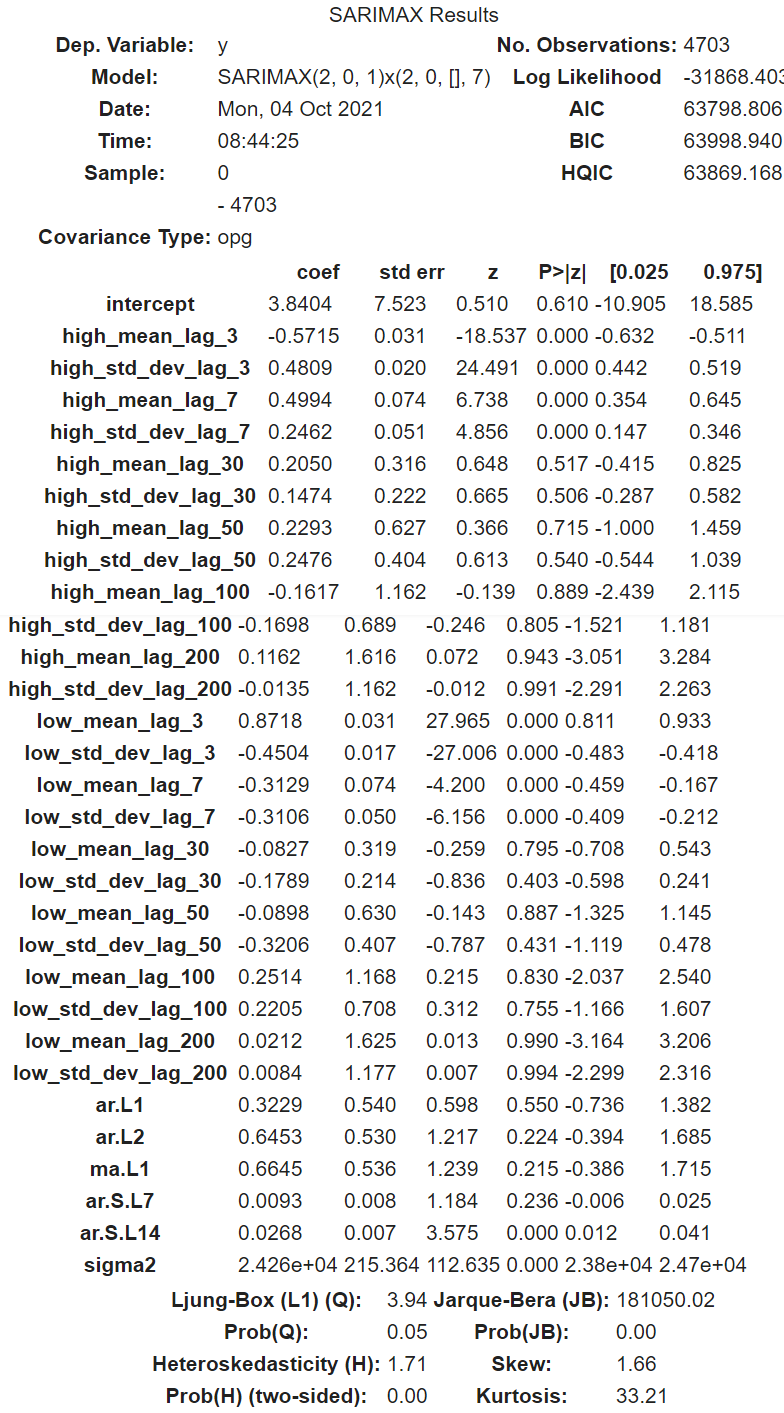
\includegraphics[width = 0.75 \textwidth]{images/SENSEX-SARIMAX-Estimating-Parameters-Results.png}
    \caption{Parameter Estimation Results of SARIMAX Model for S\&P BSE SENSEX}
    \label{fig:sensex_sarimax_parameter_estimation_report}
\end{figure}

\begin{table}[htbp]
    \setlength{\tabcolsep}{20pt}
    \renewcommand{\arraystretch}{1.2}
    \centering
    \caption{Hyperparameter Optimization Results for S\&P-500 $SARIMAX(p, d, q) \times (P, D, Q)[m]$}
    \begin{tabular}{|c|c|c|c|}
        \hline
        Sr. No & Model Parameters & AIC & Time Taken (In Seconds) \\
        \hline
        1 &  $SARIMAX(2, 1, 2) \times (1, 0, 1)[7]$ & $\infty$ & $83.16 \; sec$ \\
        \hline
        2 &  $SARIMAX(0, 1, 0) \times (0, 0, 0)[7]$ & $38148.431$ & $3.34 \; sec$ \\
        \hline
        3 &  $SARIMAX(1, 1, 0) \times (1, 0, 0)[7]$ & $37982.573$ & $31.96 \; sec$ \\
        \hline
        4 &  $SARIMAX(0, 1, 1) \times (0, 0, 1)[7]$ & $\infty$ & $64.71 \; sec$ \\
        \hline
        5 &  $SARIMAX(0, 1, 0) \times (0, 0, 0)[7]$ & $38146.500$ & $10.57 \; sec$ \\
        \hline
        6 &  $SARIMAX(1, 1, 0) \times (0, 0, 0)[7]$ & $37980.907$ & $13.22 \; sec$ \\
        \hline
        7 &  $SARIMAX(1, 1, 0) \times (0, 0, 1)[7]$ & $37982.527$ & $31.14 \; sec$ \\
        \hline
        8 &  $SARIMAX(1, 1, 0) \times (1, 0, 1)[7]$ & $37979.830$ & $61.67 \; sec$ \\
        \hline
        9 &  $SARIMAX(1, 1, 0) \times (2, 0, 1)[7]$ & $37966.387$ & $90.55 \; sec$ \\
        \hline
        10 &  $SARIMAX(1, 1, 0) \times (2, 0, 0)[7]$ & $37968.068$ & $54.21 \; sec$ \\
        \hline
        11 &  $SARIMAX(1, 1, 0) \times (2, 0, 2)[7]$ & $37966.804$ & $94.59 \; sec$ \\
        \hline
        12 &  $SARIMAX(1, 1, 0) \times (0, 0, 2)[7]$ & $37967.801$ & $51.95 \; sec$ \\
        \hline
        13 &  $SARIMAX(0, 1, 0) \times (1, 0, 2)[7]$ & $38134.564$ & $69.64 \; sec$ \\
        \hline
        14 &  $SARIMAX(2, 1, 0) \times (1, 0, 2)[7]$ & $37287.588$ & $102.89 \; sec$ \\
        \hline
        13 &  $SARIMAX(2, 1, 0) \times (0, 0, 2)[7]$ & $37286.856$ & $63.81 \; sec$ \\
        \hline
        14 &  $SARIMAX(2, 1, 0) \times (0, 0, 1)[7]$ & $37293.956$ & $41.52 \; sec$ \\
        \hline
        15 &  $SARIMAX(2, 1, 0) \times (1, 0, 1)[7]$ & $37294.387$ & $70.85 \; sec$ \\
        \hline
        16 &  $SARIMAX(3, 1, 0) \times (0, 0, 2)[7]$ & $37174.250$ & $81.39 \; sec$ \\
        \hline
        17 &  $SARIMAX(3, 1, 0) \times (0, 0, 1)[7]$ & $37178.919$ & $52.61 \; sec$ \\
        \hline
        18 &  $SARIMAX(3, 1, 0) \times (1, 0, 2)[7]$ & $37172.849$ & $101.35 \; sec$ \\
        \hline
        19 &  $SARIMAX(3, 1, 0) \times (1, 0, 1)[7]$ & $37179.242$ & $80.03 \; sec$ \\
        \hline
        20 &  $SARIMAX(3, 1, 0) \times (2, 0, 2)[7]$ & $37175.935$ & $138.21 \; sec$ \\
        \hline
        21 &  $SARIMAX(3, 1, 0) \times (2, 0, 1)[7]$ & $37173.311$ & $126.11 \; sec$ \\
        \hline
        22 &  $SARIMAX(4, 1, 0) \times (1, 0, 2)[7]$ & $36860.662$ & $97.76 \; sec$ \\
        \hline
        23 &  $SARIMAX(4, 1, 0) \times (0, 0, 2)[7]$ & $36861.244$ & $97.09 \; sec$ \\
        \hline
        24 &  $SARIMAX(4, 1, 0) \times (1, 0, 1)[7]$ & $36862.660$ & $79.44 \; sec$ \\
        \hline
        25 &  $SARIMAX(4, 1, 0) \times (2, 0, 2)[7]$ & $36862.021$ & $153.08 \; sec$ \\
        \hline
        26 &  $SARIMAX(4, 1, 0) \times (0, 0, 1)[7]$ & $36862.779$ & $62.49 \; sec$ \\
        \hline
        27 &  $SARIMAX(4, 1, 0) \times (2, 0, 1)[7]$ & $36859.024$ & $154.65 \; sec$ \\
        \hline
        28 &  $SARIMAX(4, 1, 0) \times (2, 0, 0)[7]$ & $36860.098$ & $135.74 \; sec$ \\
        \hline
        29 &  $SARIMAX(4, 1, 0) \times (1, 0, 0)[7]$ & $36864.656$ & $68.69 \; sec$ \\
        \hline
        30 &  $SARIMAX(5, 1, 0) \times (2, 0, 1)[7]$ & $36687.494$ & $145.83 \; sec$ \\
        \hline
        31 &  $SARIMAX(5, 1, 0) \times (1, 0, 1)[7]$ & $36691.327$ & $90.89 \; sec$ \\
        \hline
        32 &  $SARIMAX(5, 1, 0) \times (2, 0, 0)[7]$ & $36686.353$ & $143.59 \; sec$ \\
        \hline
        33 &  $SARIMAX(5, 1, 0) \times (1, 0, 0)[7]$ & $36689.304$ & $89.38 \; sec$ \\
        \hline
        34 &  $SARIMAX(5, 1, 1) \times (2, 0, 0)[7]$ & $35705.968$ & $153.36 \; sec$ \\
        \hline
        35 &  $SARIMAX(5, 1, 1) \times (1, 0, 0)[7]$ & $35709.171$ & $96.57 \; sec$ \\
        \hline
        \textbf{36} &  $SARIMAX(5, 1, 1) \times (2, 0, 1)[7]$ & $35713.686$ & $169.14 \; sec$ \\
        \hline
        37 &  $SARIMAX(5, 1, 1) \times (1, 0, 1)[7]$ & $35712.920$ & $97.47 \; sec$ \\
        \hline
        38 &  $SARIMAX(4, 1, 2) \times (2, 0, 0)[7]$ & $\infty$ & $166.30 \; sec$ \\
        \hline
        39 &  $SARIMAX(5, 1, 2) \times (2, 0, 0)[7]$ & $35835.432$ & $180.22 \; sec$ \\
        \hline
        40 &  $SARIMAX(4, 1, 2) \times (2, 0, 0)[7]$ & $\infty$ & $189.24 \; sec$ \\
        \hline
        41 &  $SARIMAX(5, 1, 1) \times (2, 0, 0)[7]$ & $35701.821$ & $155.03 \; sec$ \\
        \hline
        42 &  $SARIMAX(5, 1, 1) \times (1, 0, 0)[7]$ & $35704.085$ & $102.28 \; sec$ \\
        \hline
        43 &  $SARIMAX(5, 1, 1) \times (2, 0, 1)[7]$ & $35701.260$ & $169.10 \; sec$ \\
        \hline
        44 &  $SARIMAX(5, 1, 1) \times (1, 0, 1)[7]$ & $35714.812$ & $103.18 \; sec$ \\
        \hline
        45 &  $SARIMAX(5, 1, 1) \times (2, 0, 2)[7]$ & $35704.473$ & $166.71 \; sec$ \\
        \hline
        46 &  $SARIMAX(5, 1, 1) \times (1, 0, 2)[7]$ & $35704.084$ & $145.28 \; sec$ \\
        \hline
        47 &  $SARIMAX(4, 1, 1) \times (2, 0, 1)[7]$ & $\infty$ & $164.34 \; sec$ \\
        \hline
        48 &  $SARIMAX(5, 1, 0) \times (2, 0, 1)[7]$ & $36684.824$ & $154.38 \; sec$ \\
        \hline
        49 &  $SARIMAX(5, 1, 2) \times (2, 0, 1)[7]$ & $35815.786$ & $164.77 \; sec$ \\
        \hline
        50 &  $SARIMAX(4, 1, 0) \times (2, 0, 1)[7]$ & $36857.435$ & $164.84 \; sec$ \\
        \hline
        51 &  $SARIMAX(4, 1, 2) \times (2, 0, 1)[7]$ & $\infty$ & $179.75 \; sec$ \\
        \hline
    \end{tabular}
    \label{tab:s_and_p_500_hyperparameters_tunning_results_table}
\end{table}

The best model for S\&P-500 on the basis of AIC values is $SARIMAX(5, 1, 1) \times (2, 0, 1)[7]$.

\begin{figure}[htbp]
    \centering
    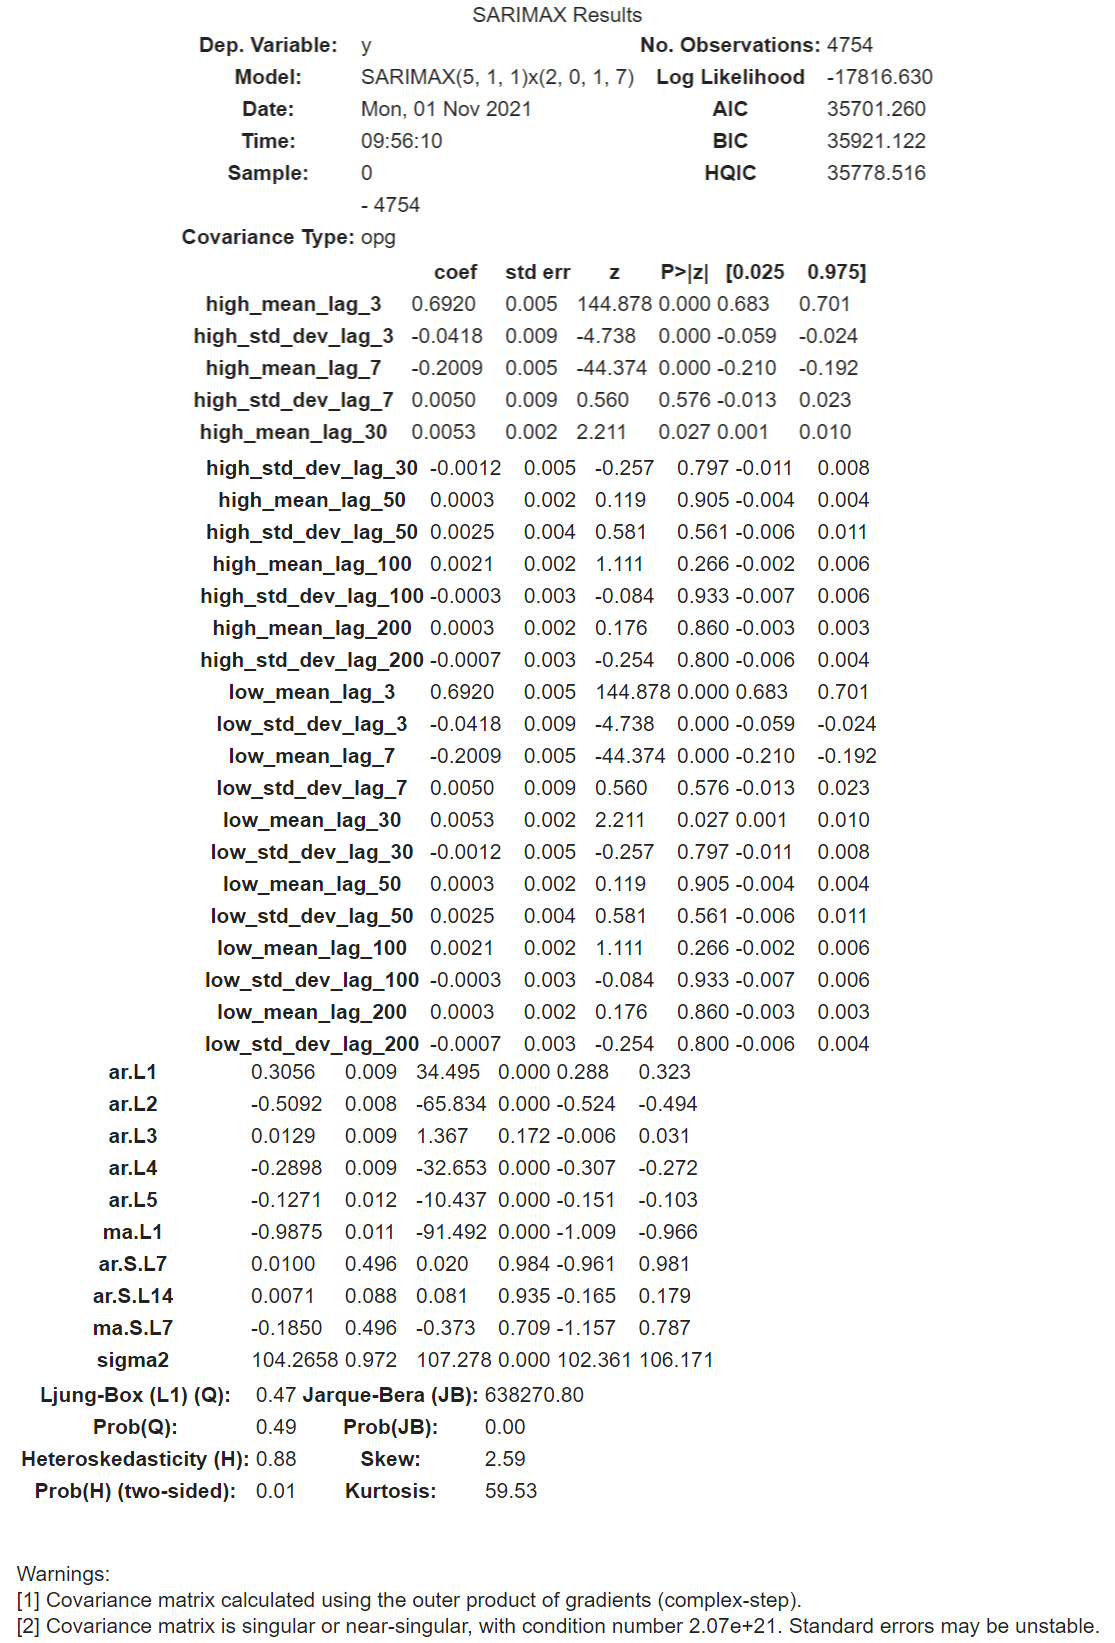
\includegraphics[width = 0.90\textwidth]{images/S&P-500-Parameter-Estimation-Results.png}
    \caption{Parameter Estimation Results of SARIMAX Model for S\&P-500.}
    \label{fig:s_and_p_500_parameter_estimation_report}
\end{figure}

\end{document}